% Adaptive Gain Evolution
% TikZ diagram for Chapter 5 - Real-time gain adaptation

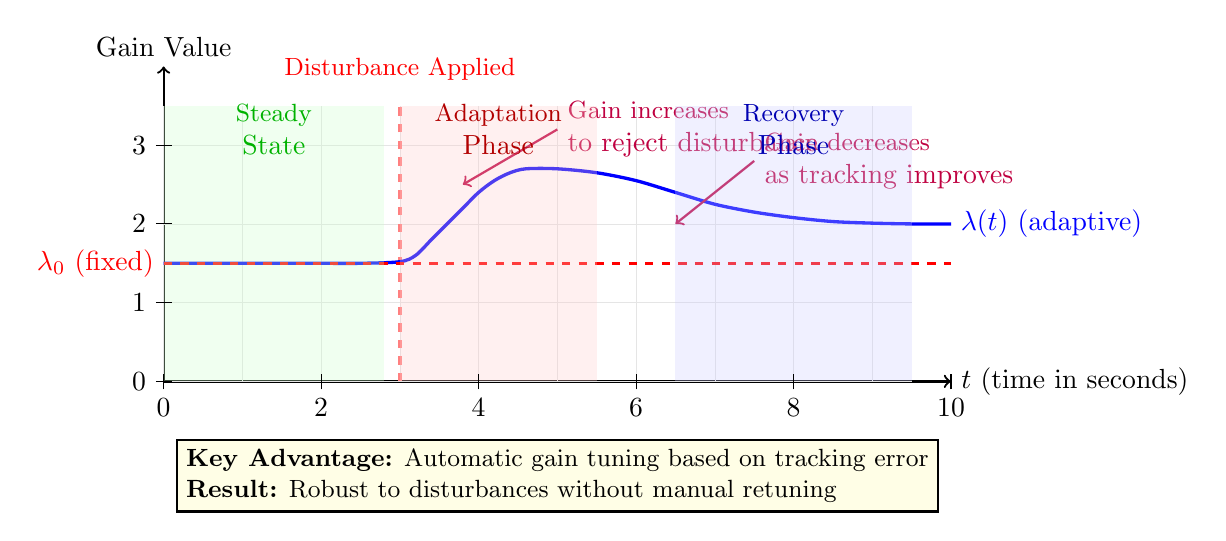
\begin{tikzpicture}[scale=1.0]

    % Axes
    \draw[->, thick] (0, 0) -- (10, 0) node[right] {$t$ (time in seconds)};
    \draw[->, thick] (0, 0) -- (0, 4) node[above] {Gain Value};

    % Grid
    \draw[gray!20, very thin] (0, 0) grid (9.5, 3.5);

    % Disturbance event marker
    \draw[red!50, very thick, dashed] (3, 0) -- (3, 3.5);
    \node[red, above] at (3, 3.7) {\small Disturbance Applied};

    % Adaptive gain $\lambda$ (responds to disturbance) - using coordinates to avoid TikZ dimension errors
    \draw[blue, very thick, smooth] plot coordinates {
        (0,1.5) (0.5,1.5) (1,1.5) (1.5,1.5) (2,1.5) (2.5,1.5)
        (3,1.52) (3.2,1.6) (3.4,1.8) (3.6,2.0) (3.8,2.2) (4,2.4)
        (4.2,2.55) (4.4,2.65) (4.6,2.7) (5,2.7) (5.5,2.65)
        (6,2.55) (6.5,2.4) (7,2.25) (7.5,2.15) (8,2.08)
        (8.5,2.03) (9,2.01) (9.5,2.0) (10,2.0)
    };
    \node[blue, right] at (10, 2.0) {$\lambda(t)$ (adaptive)};

    % Fixed gain (constant)
    \draw[red, dashed, very thick] (0, 1.5) -- (10, 1.5);
    \node[red, left] at (0, 1.5) {$\lambda_0$ (fixed)};

    % Annotations
    \draw[<-, thick, purple] (3.8, 2.5) -- (5, 3.2)
        node[right, align=left] {\small Gain increases\\to reject disturbance};

    \draw[<-, thick, purple] (6.5, 2.0) -- (7.5, 2.8)
        node[right, align=left] {\small Gain decreases\\as tracking improves};

    % Performance regions
    \fill[green!20, opacity=0.3] (0, 0) rectangle (2.8, 3.5);
    \node[green!70!black, align=center] at (1.4, 3.2) {\small Steady\\State};

    \fill[red!20, opacity=0.3] (3, 0) rectangle (5.5, 3.5);
    \node[red!70!black, align=center] at (4.25, 3.2) {\small Adaptation\\Phase};

    \fill[blue!20, opacity=0.3] (6.5, 0) rectangle (9.5, 3.5);
    \node[blue!70!black, align=center] at (8, 3.2) {\small Recovery\\Phase};

    % Tick marks
    \foreach \x in {0, 2, 4, 6, 8, 10}
        \draw (\x, -0.1) -- (\x, 0.1) node[below, yshift=-2mm] {$\x$};
    \foreach \y in {0, 1, 2, 3}
        \draw (-0.1, \y) -- (0.1, \y) node[left, xshift=-2mm] {$\y$};

    % Comparison box
    \node[draw, thick, fill=yellow!10, align=left, font=\small] at (5, -1.2) {
        \textbf{Key Advantage:} Automatic gain tuning based on tracking error\\
        \textbf{Result:} Robust to disturbances without manual retuning
    };

\end{tikzpicture}
